\section{全微分的几何意义}

本节是对矢量、全微分和隐函数求导的汇总型应用,是空间矢量和微分的第一次结合,熟练掌握和细品。

本节要点:
\begin{itemize}
    \item 深入理解全微分的几何意义;
    \item 深入理解方向导数的概念。
\end{itemize}

%============================================================
\subsection{空间曲线的切线和法平面}

\begin{figure}[h]
\centering
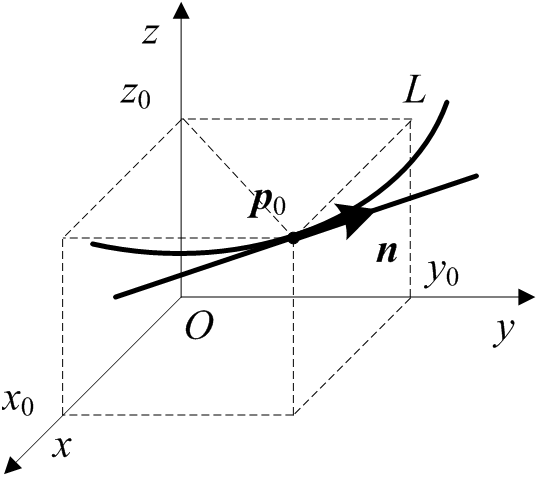
\includegraphics[height=4cm]{7.2.png}
\end{figure}

\begin{definition}
设三维空间的曲线
\[
L:\left\{ \begin{array}{c}
	x=x\left( t \right)\\
	y=y\left( t \right)\\
	z=z\left( t \right)\\
\end{array} \right.
\]
则曲线在点$\boldsymbol{p}_0$处(即对应$t_0$)的切线的方向称为{\bf 曲线$L$的切向量},假设记为$\boldsymbol{n}$,则有:
\[
\boldsymbol{n}=\left. \left( \begin{array}{c}
	x'\\
	y'\\
	z'\\
\end{array} \right) \right|_{t=t_0}=\left( \begin{array}{c}
	x'\left( t_0 \right)\\
	y'\left( t_0 \right)\\
	z'\left( t_0 \right)\\
\end{array} \right)
\]
于是,曲线$L$在点$\boldsymbol{p}_0$处的切线方程为$\boldsymbol{p}-\boldsymbol{p}_0=\lambda \boldsymbol{n}$,展开后为:
\[
\left( \begin{array}{c}
	x\\
	y\\
	z\\
\end{array} \right) -\left( \begin{array}{c}
	x_0\\
	y_0\\
	z_0\\
\end{array} \right) =\lambda \left( \begin{array}{c}
	x'\left( t_0 \right)\\
	y'\left( t_0 \right)\\
	z'\left( t_0 \right)\\
\end{array} \right) \quad \text{或} \quad \frac{x-x_0}{x'\left( t_0 \right)}=\frac{y-y_0}{y'\left( t_0 \right)}=\frac{z-z_0}{z'\left( t_0 \right)}
\]
过点$\boldsymbol{p}_0$垂直于该点切线的平面称为{\bf 曲线$L$在点$\boldsymbol{p}_0$处的法平面},法平面方程为$\left( \boldsymbol{p}-\boldsymbol{p}_0 \right) ^T\boldsymbol{n}=0$,展开后为:
\[
\left( x-x_0 \right) \cdot x'\left( t_0 \right) +\left( y-y_0 \right) \cdot y'\left( t_0 \right) +\left( z-z_0 \right) \cdot z'\left( t_0 \right) =0
\]
\end{definition}

如果曲线由两个平面
\[
L:\left\{ \begin{array}{c}
	F\left( x,y,z \right) =0\\
	G\left( x,y,z \right) =0\\
\end{array} \right.
\]
相交而成,则在点$\boldsymbol{p}_0$处的切向量为:
\[
\boldsymbol{n}=\left. \left( 1\,\,\frac{\partial y}{\partial x}\,\,\frac{\partial z}{\partial x} \right) ^T \right|_{\boldsymbol{p}_0}
\]
切线方程为:
\[
\frac{x-x_0}{1}=\frac{y-y_0}{\left. \frac{\partial y}{\partial x} \right|_{\boldsymbol{p}_0}}=\frac{z-z_0}{\left. \frac{\partial z}{\partial x} \right|_{\boldsymbol{p}_0}}
\]
法平面方程为:
\[
\left( x-x_0 \right) +\left( y-y_0 \right) \cdot \left. \frac{\partial y}{\partial x} \right|_{\boldsymbol{p}_0}+\left( z-z_0 \right) \cdot \left. \frac{\partial z}{\partial x} \right|_{\boldsymbol{p}_0}=0
\]

%============================================================
\subsection{空间曲面的切平面和法线}

\begin{figure}[h]
\centering
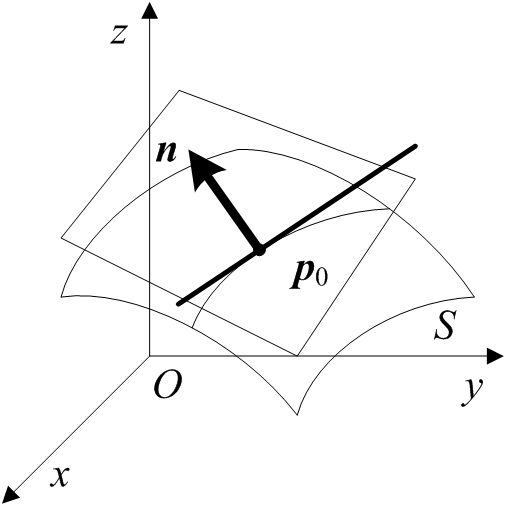
\includegraphics[height=4cm]{7.3.png}
\end{figure}

\begin{definition}
若曲面$S$由方程$F\left( \boldsymbol{p} \right) =0,\boldsymbol{p}=\left( x\,\,y\,\,z \right) ^T$隐式给出,对于在点$\boldsymbol{p}_0$处垂直于切平面的方向称为{\bf 曲面$S$在$\boldsymbol{p}_0$处的法向量},假设记为$\boldsymbol{n}$,则有:
\[
\boldsymbol{n}=\left. \left( \begin{array}{c}
	F_x\\
	F_y\\
	F_z\\
\end{array} \right) \right|_{\boldsymbol{p}_0}
\]
{\bf 曲面$S$在点$\boldsymbol{p}_0$处的法线方程}为$\boldsymbol{p}-\boldsymbol{p}_0=\lambda \boldsymbol{n}$,即:
\[
\left( \begin{array}{c}
	x\\
	y\\
	z\\
\end{array} \right) -\left( \begin{array}{c}
	x_0\\
	y_0\\
	z_0\\
\end{array} \right) =\lambda \left( \begin{array}{c}
	F_x\left( \boldsymbol{p}_0 \right)\\
	F_y\left( \boldsymbol{p}_0 \right)\\
	F_z\left( \boldsymbol{p}_0 \right)\\
\end{array} \right) \quad \text{或} \quad \frac{x-x_0}{F_x\left( \boldsymbol{p}_0 \right)}=\frac{y-y_0}{F_y\left( \boldsymbol{p}_0 \right)}=\frac{z-z_0}{F_z\left( \boldsymbol{p}_0 \right)}
\]
{\bf 曲面$S$在点$\boldsymbol{p}_0$处的切平面方程}为$\left( \boldsymbol{p}-\boldsymbol{p}_0 \right) ^T\boldsymbol{n}=0$,即:
\[
\left( x-x_0 \right) \cdot F_x\left( \boldsymbol{p}_0 \right) +\left( y-y_0 \right) \cdot F_y\left( \boldsymbol{p}_0 \right) +\left( z-z_0 \right) \cdot F_z\left( \boldsymbol{p}_0 \right) =0
\]
\end{definition}

若曲面由$z=z\left( x,y \right) $显式给出,则法向量:
\[
\boldsymbol{n}=\left. \left( \begin{array}{c}
	-z_x\\
	-z_y\\
	1\\
\end{array} \right) \right|_{\boldsymbol{p}_0}
\]
法线方程:
\[
\frac{x-x_0}{-z_x\left( \boldsymbol{p}_0 \right)}=\frac{y-y_0}{-z_y\left( \boldsymbol{p}_0 \right)}=\frac{z-z_0}{1}
\]
切平面方程:
\[
-\left( x-x_0 \right) \cdot z_x\left( \boldsymbol{p}_0 \right) -\left( y-y_0 \right) \cdot z_y\left( \boldsymbol{p}_0 \right) +\left( z-z_0 \right) =0
\]

~

\begin{example}
求曲面$x^2+2y^2+3z^2=6$在$\boldsymbol{p}_0=\left( 1\,\,1\,\,1 \right) $处的切平面和法线。
\end{example}

解:

构造$F=x^2+2y^2+3z^2-6$,得$\boldsymbol{p}_0$处的法线方向:
\[
\boldsymbol{n}=\left. \left( \begin{array}{c}
	F_x\\
	F_y\\
	F_z\\
\end{array} \right) \right|_{\boldsymbol{p}_0}=\left. \left( \begin{array}{c}
	2x\\
	4y\\
	6z\\
\end{array} \right) \right|_{\boldsymbol{p}_0}=\left( \begin{array}{c}
	2\\
	4\\
	6\\
\end{array} \right)
\]
切平面和法线:
\begin{align*}
&2\left( x-1 \right) +4\left( y-1 \right) +6\left( z-1 \right) =0 \\
&\frac{x-1}{2}=\frac{y-1}{4}=\frac{z-1}{6}
\end{align*}

%============================================================
\subsection{全微分的几何意义}

根据上节的空间曲面$z=z\left( x,y \right) $的切平面方程,对比全微分,如下:
\begin{align*}
&-\left( x-x_0 \right) \cdot z_x\left( \boldsymbol{p}_0 \right) -\left( y-y_0 \right) \cdot z_y\left( \boldsymbol{p}_0 \right) +\left( z-z_0 \right) =0 \\
&dz=z_x\cdot dx+z_y\cdot dy
\end{align*}
$z=z\left( x,y \right) $在点$\boldsymbol{p}_0$处的全微分的几何意义表示曲面$S$在点$\boldsymbol{p}_0$处的切平面在{\it z}轴的增量。

全微分的几何意义体现出一点,曲面要在某一点有切平面,必须在这一点光滑——不断不折。
只有光滑了,才有切平面,才有切平面在{\it z}轴的增量。
细品!

%============================================================
\subsection{方向导数定理}

我们之前定义了方向导数
\[
\left. \frac{\partial z}{\partial n} \right|_{\boldsymbol{p}_0}=\underset{\left\| \Delta _n\boldsymbol{p} \right\| \rightarrow 0}{\lim}\frac{\Delta _nz}{\left\| \Delta _n\boldsymbol{p} \right\|}=\underset{\left\| \Delta _n\boldsymbol{p} \right\| \rightarrow 0}{\lim}\frac{f\left( \boldsymbol{p}_0+\Delta _n\boldsymbol{p} \right) -f\left( \boldsymbol{p}_0 \right)}{\left\| \Delta _n\boldsymbol{p} \right\|}
\]
但当时还没有引入全微分,我们这里用全微分完善方向导数。

\begin{theorem}[方向导数定理]
设函数$z=z\left( \boldsymbol{p} \right) $在一点处可微,则该函数在此点处存在沿任意方向$n$的方向导数,且有:
\[
\frac{\partial z}{\partial n}=\frac{\partial z}{\partial x}\cos \alpha +\frac{\partial z}{\partial y}\cos \beta
\]
其中,$\mathbf{n}=\left( \cos \alpha \,\,\cos \beta \right) ^T$为方向$n$的方向余弦。
\end{theorem}

该定理给方向导数的计算提供了方法,即如果知道一个方向,就能知道沿该方向的方向导数。

同样,对于三元函数$u=u\left( \boldsymbol{p} \right) ,\boldsymbol{p}\in \mathbb{R} ^3$,方向导数为:
\[
\frac{\partial u}{\partial n}=\frac{\partial u}{\partial x}\cos \alpha +\frac{\partial u}{\partial y}\cos \beta +\frac{\partial u}{\partial z}\cos \gamma
\]

~

\begin{example}
求函数$z=xe^{2y}$在点$\boldsymbol{p}_0=\left( 1\,\,0 \right) ^T$处,沿射线$\left( 1\,\,0 \right) ^T\rightarrow \left( 2\,\,-1 \right) ^T$的方向导数。
\end{example}

解:

首先求得偏导:
\[
\left. \left( \frac{\partial z}{\partial x}\,\,\frac{\partial z}{\partial y} \right) ^T \right|_{\boldsymbol{p}_0}=\left. \left( e^{2y} \quad 2xe^{2y} \right) ^T \right|_{\boldsymbol{p}_0}=\left( 1\,\,2 \right) ^T
\]
再求射线的方向余弦:
\begin{align*}
&\because \Delta _n\boldsymbol{p}=\left( \begin{array}{c}
	2\\
	-1\\
\end{array} \right) -\left( \begin{array}{c}
	1\\
	0\\
\end{array} \right) =\left( \begin{array}{c}
	1\\
	-1\\
\end{array} \right)
\\
&\therefore \left\| \Delta _n\boldsymbol{p} \right\| =\sqrt{2} \\
&\therefore \mathbf{\theta }=\left( \frac{1}{\sqrt{2}}\,\,\frac{-1}{\sqrt{2}} \right) ^T
\end{align*}
最终,方向导数:
\[
\left. \frac{\partial z}{\partial n} \right|_{\boldsymbol{p}_0}=\left( 1\,\,2 \right) \left( \frac{1}{\sqrt{2}}\,\,\frac{-1}{\sqrt{2}} \right) ^T=\frac{1}{\sqrt{2}}+\frac{-2}{\sqrt{2}}=-\frac{1}{\sqrt{2}}
\]




